\chapter{Architecture}
\label{cha:architecture}

\todo{Blegh!...}This chapter introduces the architecture of the new tile that has been developed. 

\section{Hashing tile with DMA module}

For this project, a new tile has been made for SHMAC, which can be seen in figure \ref{fig:SHA-Tile}.

\begin{figure}[htb]
    \centering
    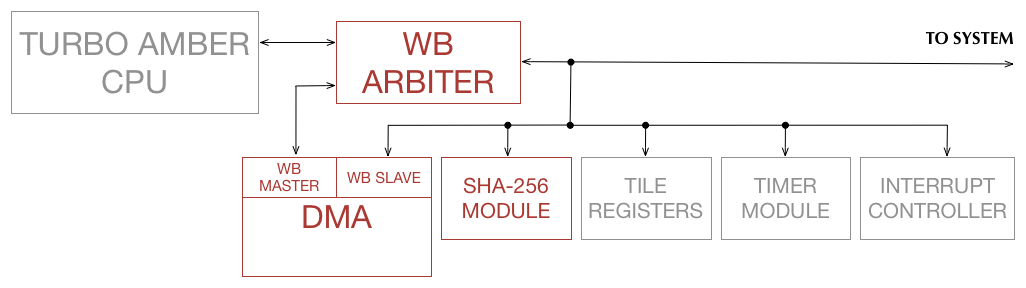
\includegraphics[width=1.0\textwidth]{Figures/Tile/HashingTile}
    \caption{New SHMAC-tile, consisting of a unique SHA-256 hashing tile, a DMA Module and a Wishbone Arbiter.}
    \label{fig:SHA-Tile}
\end{figure}

The tile is based on the Turbo Amber tile, which consists of a Turbo Amber core, tile registers, timer module and interrupt controller.
The new components for this tile are the SHA-256 hashing module, the DMA Module, and the Wishbone Bus Arbiter, all marked in red.

\subsection{SHA-256 Hashing Module}
\todo{KRISTIAAAAAAAAANN!!!!!}HÆSJÆSJÆSJÆSJ!!!


\subsection{DMA Module}
Originally made for the \todo{would need a reference} project during the Autumn 2014 at NTNU, the DMA Module has been modified further for use in this project.
It can be seen in figure \ref{fig:DMATop}.

\begin{figure}[htb]
    \centering
    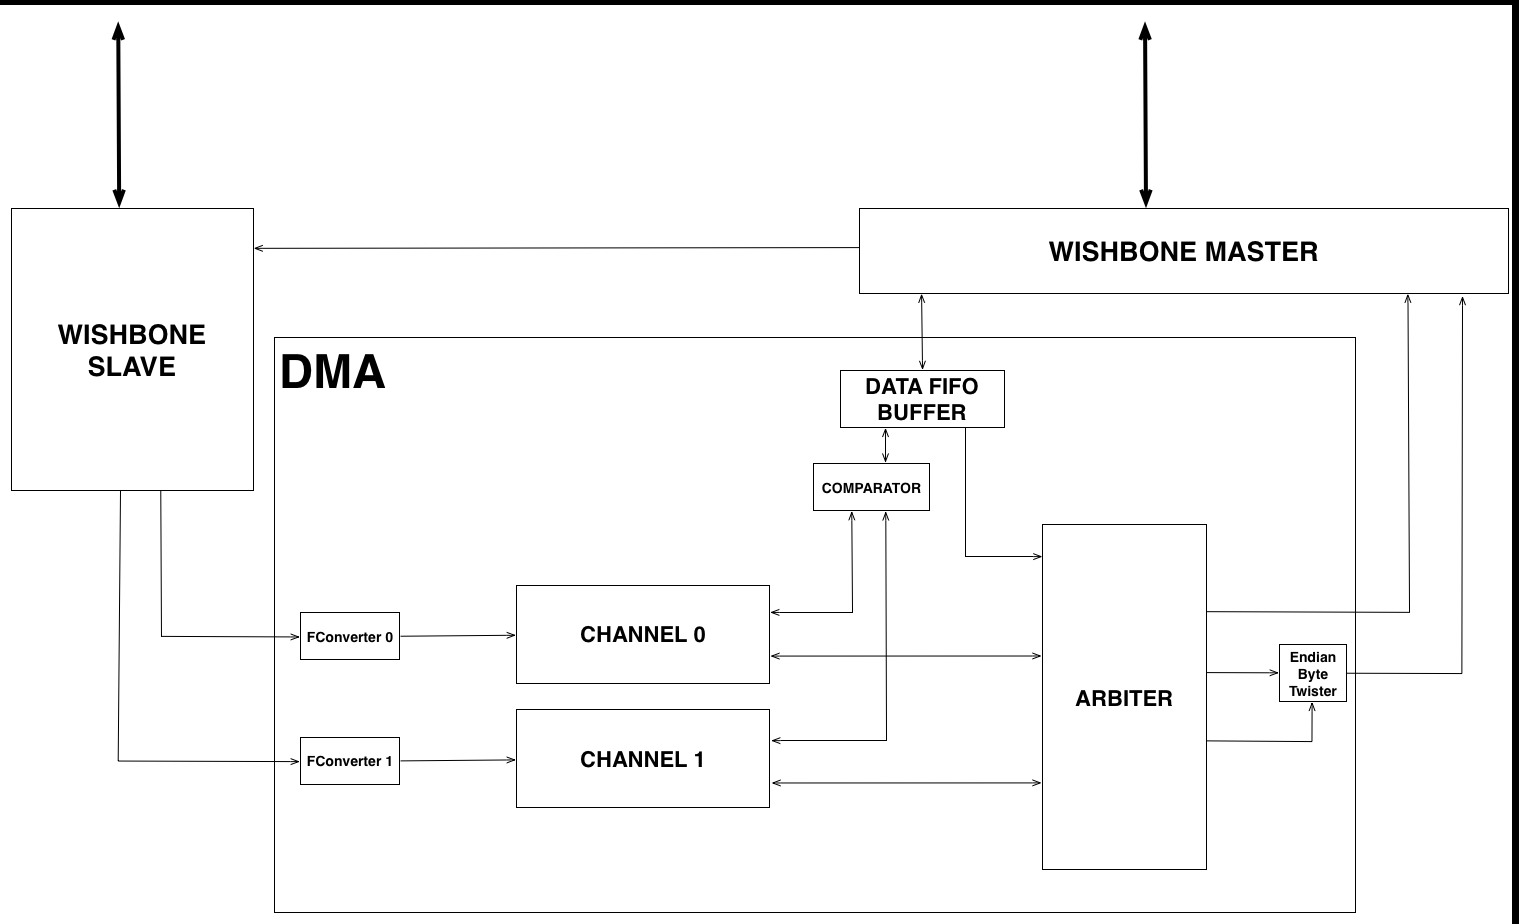
\includegraphics[width=1.0\textwidth]{Figures/DMA/DMATopview}
    \caption{DMA Topview, including Wishbone interface.}
    \label{fig:DMATop}
\end{figure}

The DMA module was made as part of the project to test if separate data transfers with a DMA module could improve performance and energy efficiency in the Hashing process, leveraging the tile CPU for other work and specializing this module more efficiently for data transfer.

The DMA consists of three submodules: Wishbone Slave for receiving transfer requests, Wishbone Master for interfacing data transfer with the Wishbone bus system, and the DMA module itself, which generates the individual transfer commands.

\todo{The 14th commandment: Thou shall satisfy Kristian. The 13th commandment: Thou shall satisfy ME!!!}The Wishbone Slave consists of three registers for each DMA Channel, making it six in total.
The registers are used for base source, base destination and detailing the transfer request.
When request is activated, the selected channel receives data from the slave, and executes the transfer.
An arbiter selects commands from the channels if both are active.
Every single command from the channels are passed on to the Wishbone master, which executes the command.
The command is either a load or a store command.
Any received data from a load command is passed on to the correct channel, and when a channel if finished, the imformation is passed from the Wishbone Master to the Wishbone Slave, so it can modify its registers and interrupt the CPU. 

\todo{Denne SKA med}In addition for this project, the DMA Module also has submodule for endian byte switching, since the results from the SHA-256 hashing process is stored with lowest endian byte first.
Switching the bytes instantly as they pass through the submodule should be more efficient than in software, since the software solution would require to \todo{Either put in example, or set in reference to software solution that does not use DMA, when it is added to the report.}load the data and shift the bytes for each existing byte.

\subsection{Wishbone Arbiter}
With the presence of a Wishbone Master in the DMA Module, the tile has now two masters that will demand access to the shared Wishbone bus network. 
Arbritation is therefore required.

For this project, the ARB0001a: 4 Level, Round-robin Arbiter from WISHBONE Public Domain Library for VHDL has been taken in use.
Figure \cite{fig:WBArbiter} shows how the arbitration works, with Round-robin.
The arbiter will in turn check each input master for bus requests, and grants access thereby.
If a master has no request, the arbiter will continue to the next.
For this project, only two masters are present.
Arbitration normally take a full clock cycle.
See \cite{WBLibrary} for detailed implementation.

\begin{figure}[htb]
    \centering
    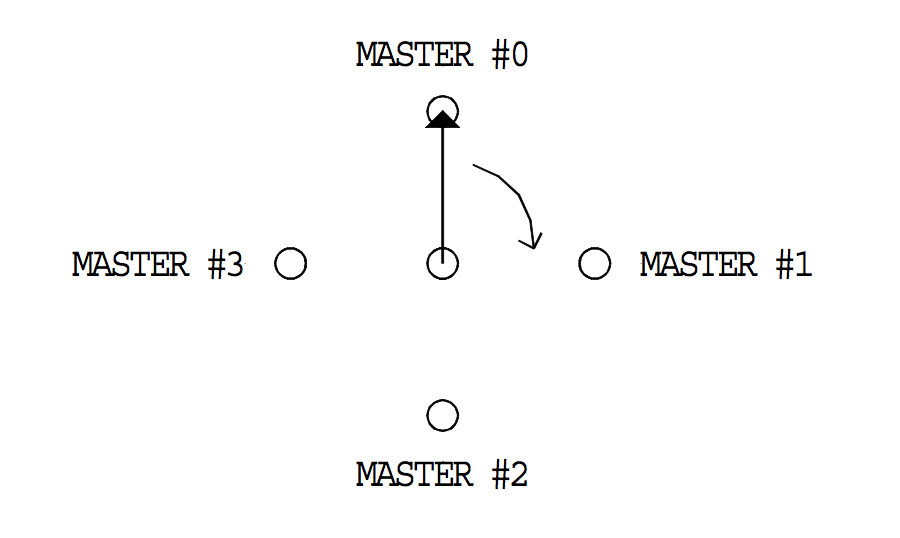
\includegraphics[width=1.0\textwidth]{Figures/Tile/WBArbiter}
    \caption{Wishbone Round-robin Arbiter, as seen in \cite{WBLibrary}.}
    \label{fig:WBArbiter}
\end{figure}

\todo{Discussion of alternatives. The following may be moved to future work.}Round-robin arbiters work well in data acquisition systems where data is collected and placed into shared memory, since peripherals must often off-load data to memory on an equal basis.
The choice of this arbiter is due to using an already established Wishbone arbiter cuts away time from designing a new one, \todo{Hmm.... Sounds uncalled for}which may even end up less efficient in worse case.
An alternative to round-robin arbiters is priority arbiters.
They are usually disadvantagous in said systems, but does not have the arbitration overhead \cite{WBLibrary}.

In the case of arbitration between a CPU and a DMA Module, a priority arbiter may be used to achieve either burst mode, where DMA gets the full right on the bus until the transfer is finished, or transparent mode, where the CPU always has first right.
The latter mode gives the slowest DMA transfer, but has shown to give best overall system performance. \todo{Find those book sources again, if time. Current source does not validate claim of overall performance} \cite{DMA-lecture}.

